\chapter{Cahier des besoins}\label{cahier-des-besoins}

\section{Besoins fonctionnels}\label{besoins-fonctionnels}

\subsection{Algorithme de CDLOD sur terrain sphérique}\label{algorithme-de-cdlod}

Implémenter l'algorithme de CDLOD expliqué dans le chapitre \ref{chap:cdlod} de F.
Strugar~\cite{CDLOD}, sur un terrain sphérique:\\

  \begin{figure}[!ht]
  \centerline{
    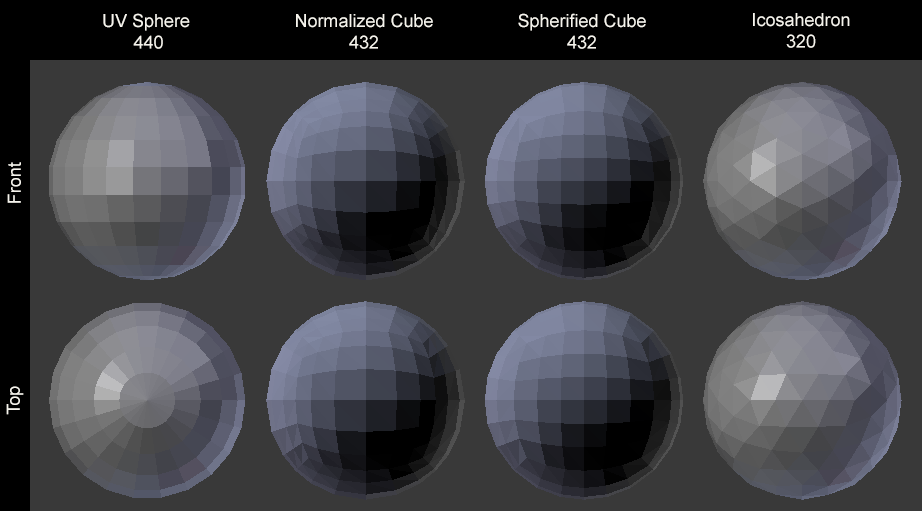
\includegraphics[width=12cm]{img/spheres.png}}
     \caption[Sphère génération]{Différentes manières de former le maillage d'une sphère, avec le nombre de triangles associé.\protect\footnotemark}
    \label{fig:spheres}
    \end{figure}
\footnotetext{Extrait de \url{https://github.com/caosdoar/spheres/tree/master/},
dernier accès: avril 2018}

\begin{itemize}
\item 
  Former un terrain sphérique. La sphère sera approximée à l'aide d'un
    maillage géométrique à base de triangles. Plusieurs méthodes sont
    disponibles pour générer une sphère à partir de triangles (ou de
    rectangles composés de deux triangles).
  \begin{itemize}
  \item
    UV Sphere: Générer la sphère en plaçant les points le long des
      méridiens et parallèles. Cette technique est simple mais les faces
      de la sphère ne sont pas toutes égales, ce qui ne place pas les
      points de manière uniforme sur la surface de la sphère, posant
      problème lors de la découpe du terrain dans le \emph{quadtree}
      (voir~\ref{sec:quadtree}).
  \item
    Déformation de cube: Générer le maillage d'un cube puis le déformer en
      gonflant ses faces. Le cube peut être déformé de plusieurs manières,
      cependant les faces de la sphère ne sont là encore jamais
      parfaitement égales.
  \item
    Subdivision d'icosaèdre: Former un icosaèdre (polyèdre à 20 faces
      triangulaires égales) puis subdiviser chaque face en quatre autres
      triangles égaux (voir~\ref{subsec:icosaèdre}). Le maillage qui en
      résulte est uniforme.
  \end{itemize}

\item
  Gérer les informations de détails du terrain sous forme de
    \emph{quadtree}~\ref{sec:quadtree}. Parcourir le \emph{quadtree} permettra de
    générer le maillage de la sphère par rapport à la distance de chaque
    noeud à la caméra.
\item
  Effectuer un \emph{morphing} entre deux niveaux de détails afin de
    lisser les transitions entre les deux niveaux~\ref{subsec:morphing}. La
    taille du \emph{morphing} ainsi que sa position sont déterminées en
    fonction du niveau de détail. Plus le niveau de détails est bas, plus il est profond dans l'arbre, plus détaillé (niveaux LOD0, LOD1).
\end{itemize}

Cette partie est complexe et devrait nécessiter quatre semaines de travail.

\subsection{Interface graphique}\label{interface-graphique}

Proposer une interface graphique afin de voir l'effet de l'algorithme
sur un maillage. L'interface est composée d'un rendu "temps réel" du
maillage de la planète, et d'un affichage d'informations complémentaires
comportant le nombre de triangles actuellement affiché à l'écran ainsi
que le nombre d'images générées par seconde. L'utilisateur doit pouvoir
déplacer la caméra autour de la planète à l'aide du clavier et
l'orienter à la souris.\\

Cette partie est simple et ne devrait nécessiter qu'une semaine de travail.

\subsection{Génération procédurale}\label{generation-procedurale}

Générer procéduralement le terrain de la planète, en proposant un choix
de la méthode de génération de la carte de hauteur. Le choix de la
méthode se fait en option de lancement du programme. L'utilisateur entre le nom de la méthode de génération, ainsi que les paramètres associés. Les paramètres varient en fonction de la méthode, cependant certains paramètres sont toujours disponibles:
\begin{itemize}
    \item La taille de la carte;
    \item La hauteur maximale d'un sommet.
\end{itemize}

Cette partie est plutôt complexe, le temps de développement devrait être de des à trois semaines.

\section{Besoins non fonctionnels}\label{besoins-non-fonctionnels}

\subsection{Langage de programmation}

Suite aux demandes du client, le projet doit être implémenté en C++11/14
. Utiliser ces standards implique d'utiliser des compilateurs
compatibles. Voici les versions minimales à respecter pour les
compilateurs GCC et Clang (les deux plus gros compilateurs pour la
plateforme cible --- Linux):

\begin{longtable}[]{@{}lll@{}}
\toprule
Compilateur & ISO C++ & Version minimale\tabularnewline
\midrule
\endhead
GCC & C++11 & 4.8.1\tabularnewline
GCC & C++14 & 5.0\tabularnewline
Clang & C++11 & 3.3\tabularnewline
Clang & C++14 & 3.4\tabularnewline
\bottomrule
\end{longtable}

\subsection{Interface de programmation}

%Le client requiert que la version d'OpenGL soit au maximum 3.3
%afin que le projet fonctionne sur une machine avec un driver libre\footnote{\url{https://mesamatrix.net/}}.
Le client requiert que le programme fonctionne sous Linux avec des drivers graphiques libres.
Selon le site \url{https://mesamatrix.net/}, la version d'OpenGL la plus récente supportée
par tous les drivers libres est OpenGL 3.3.
PlanetRenderer étant prévu pour OpenGL 4.5, certaines modifications
seront nécessaires. Après étude des fonctions OpenGL utilisées dans le
projet, le portage ne s'avère pas difficile. Ce portage sera étudié plus
loin.

\subsection{Système de compilation}

Une dernière demande du client sur l'implémentation du projet est
d'utiliser CMake\footnote{\url{https://cmake.org/}} comme système de
compilation. PlanetRenderer étant basé sur GENie\footnote{\url{https://github.com/bkaradzic/GENie}},
il faudra porter le projet vers CMake. Cela implique de réécrire
totalement le système de compilation.

\subsection{Performances}

L’objectif du projet étant de tester les performances d’une implémentation
de Filip Strugar~\cite{CDLOD}, il n’y a pas de contrainte de performance imposée
par le client. Mais étant donné que l'application est une application de rendu en temps interactif le rendu
doit être fluide, c'est-à-dire à au moins 60 images par seconde. 
D'après nos premiers tests PlanetRenderer respecte ce besoin en étant capable
d'afficher 120 000 triangles à 60 images par seconde sur une carte
graphique Nvidia GTX 960M. Nous pouvons prévoir grâce aux études de performances de
F.Strugar l’impact de performance de l’algorithme de CDLOD. Sur
des processeurs performants de l’époque, F.Strugar mesure en moyenne
0.08ms de temps de parcours de l’arbre nécessaire pour générer le maillage
du terrain. À cela devront s’ajouter les coups de génération du maillage, ainsi
que les coups de rendu de la scène. Pour un rendu très fluide, lorsque la caméra
se déplace dans la scène, il faudrait atteindre au moins 60 images par
seconde, donc passer moins de 16ms de calcul par image. F.Strugar atteint
des performances élevées en effectuant une partie des calculs de la scène
sur GPU.



\subsection{Tests}

Des tests unitaires seront écrits sur les parties génération du maillage et parcours du quadtree, afin de s'assurer que le programme fonctionne correctement.